\documentclass[a4paper,10pt]{article}
%\usepackage[latin1]{inputenc} % Paquetes de idioma
\usepackage[utf8]{inputenc} % Paquetes de idioma (Este encoding toma acentos :) )
\usepackage[spanish]{babel} % Paquetes de idioma
\usepackage{graphicx} % Paquete para ingresar gráficos
\usepackage{grffile}
\usepackage{hyperref}
\usepackage{fancybox}
\usepackage{amsmath}
\usepackage{amsfonts}
\usepackage{listings}
\usepackage{float}
% Paquetes de macros de Circuitos
%\usepackage{pstricks}
\usepackage{tikz}

% Encabezado y Pié de página
\usepackage{fancyhdr} % Paquete para encabezados y pie de página
\pagestyle{fancy} % Sin esta línea no se imprimiría el encabezado en todas las páginas

\fancyhf{} %  Borra el encabezado anterior (Por defecto escribe el títutlo de la sección en la que se encuentra la hoja
\setlength{\headheight}{22.55pt}
\fancyhead[L]{
	{\textsf{Facultad de Ingenier\'ia $-$ Universidad de Buenos Aires \\ 66.44 Instrumentos Electrónicos}}
}
%\addtocounter{page}{5}
\fancyhead[R]{\thepage}

\renewcommand{\footrulewidth}{0.4pt} % Ajusta el tamaño de las líneas separadoras en el pié de página
\renewcommand{\headrulewidth}{0.4pt} % Ajusta el tamaño de las líneas separadoras en el encabezado

\fancyfoot[L]{
	{\textsf{Trabajo Pr\'actico N$^{\circ}4$}: Mediciones de impedancias} \\
	{\textsf{Integrantes: Eduardo Sanchez, Francisco Soler}}
	}
		

% Carátula del Trabajo
\title{ \author{} % Lo pongo para que el warning no moleste :p
\setlength{\unitlength}{1cm} %  Especifica la unidad de trabajo
\thispagestyle{empty}

\begin{picture}(18,0)
\put(0,0){
\includegraphics[width=1.5cm, height=3cm]{Logo1.png}}

\put(10.5,0){
\includegraphics[width=3cm, height=3cm]{Logo2.png}}

\end{picture}
\\[1.5cm]
\begin{center}
	\textbf{{\Huge Facultad de Ingenier\'ia \\ Universidad de Buenos Aires}}\\[2cm]
	{66.44 Instrumentos Electrónicos}\\[0.5cm]
	{Trabajo Pr\'actico N$^{\circ}3$: Mediciones de impedancias}\\[2.5cm]
\end{center}

\begin{flushleft}
	\textbf{Integrantes:} \\[1cm]

	\begin{tabular}{|c|c|c|}
		\hline
		\textbf{\normalsize Padr\'on} & \textbf{\normalsize Nombre} & \textbf{\normalsize Email} \\
		\hline
		\normalsize 92903 & \normalsize Sanchez, Eduardo Hugo & \normalsize hugo\_044@hotmail.com \\
		\hline
		\normalsize 91227 & \normalsize Soler, Jos\'e Francisco & \normalsize francisco.\_tw@hotmail.com \\
		\hline
		\normalsize xxx & \normalsize Wawrynczak, Claudio  & \normalsize claudiozak@gmail.com \\
		\hline
	\end{tabular}
\end{flushleft}
\date{} % Hace que no se imprima la fecha en la cual se compilo el .tex
 }

\begin{document}
	\maketitle % Hace que el título anterior sea el principal del documento
	\newpage

	\tableofcontents % Esta línea genera un indice a partir de las secciones y 
					 % subsecciones creadas en el documento
	\newpage


	\section{Objetivo}
	
	\indent	El objetivo del presente trabajo práctico es determinar las 
	diferentes impedancias medidas utilizando un osciloscopio con técnicas de 
	reflectometría.
	
	\newpage
	\section{Desarrollo}
\indent Para llevar a cabo las mediciones, se utilizan los siguientes
		instrumentos:
		\begin{itemize}
			\item algo
			\item algo
			\item algo
			\item Cable coaxil para realizar las distintas conexiones entre 
			instrumentos.
		\end{itemize}	
	
		\subsection{Medici\'on 1- Inductancia de una bobina usando el Q-metro}
		El circuito simplificado de un Q-metro se muestra en la Figura \ref{img001}

			\begin{figure}[!htb]
				\centering
				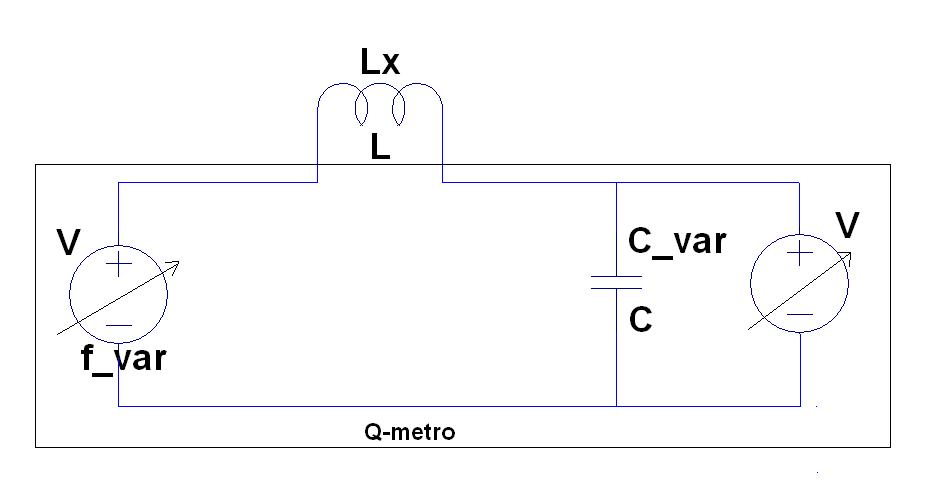
\includegraphics[width=8cm]
				{Imagenes/qmetro.png}
				\caption{Esquema simplificado del Q-metro}
				\label{img001} 
			\end{figure}
		Donde el valor m\'aximo obtenido de tensi\'on para un determinado inductor $L_x$ de inductancia $L$ se da cuando $f=\frac{1}{2\pi\sqrt{LC}}$. Por otra parte puede mostrarse que el valor de Q es $Q=\frac{\omega L}{R}$.
		
		Conocidos los valores de la capacidad, $C$, y la frecuencia, $f$, puede obtenerse el valor de la inductancia de $L_x$ y tambi\'en su resistencia serie equivalente con las siguientes expresiones
		$$L=\frac{1}{(2\pi)^2 f^2C}$$
		$$L=\frac{2\pi fL}{Q}$$
		En la tabla \ref{tab001} se muestran los resultados obtenidos para un inductor utilizando 2 frecuencias
		
		\begin{table}[!htp]
					\centering
					\begin{tabular}{|c|c|c|c|c|}
						\hline
			    		Frecuencia & C & Q & L & R \\
						\hline
						$7.9722~MHz$& $75~pF$& 200 & $5.31~\mu Hy$ &$ 1.33~\Omega$ \\
						\hline
						$13.3~MHz$& $25~pF$& 182 & $5.72~\mu Hy$ &$ 2.62~\Omega$ \\
						\hline  
					\end{tabular}
					\caption{Mediciones con el Q-metro} \label{tab001}
				\end{table}	
		\subsection{Medici\'on 2- Inductancia de una bobina usando el LCR}
		\subsection{Medici\'on 3- Inductancia de una bobina usando el puente de impedancias}
		\subsection{Medici\'on 4- Frecuencia de resonancia de una bobina}
		\subsection{Medici\'on 4- Param\'etros de una l\'inea de transmisici\'on}
		\subsection{Medici\'on 4- Inductancia de una bobina con nucleo de ferrite}
		\subsection{Medici\'on 4- Capacidad de un capacitor electro\'itico}	
		\subsection{Medici\'on 4- Capacidad de un capacitor cer\'amico}
		\subsection{Medici\'on 4- Par\'ametros de un cristal}
		\subsection{Medici\'on 4- Mediciones en un circuito activo}	
	\section{Conclusiones}
	\indent Viva Venezuela!\\
\end{document}

